The coroutines library, the modularized standard library, and the executors have something in common: they are supposed to be part of C++23.


\subsubsubsection{8.1.1\hspace{0.2cm} The Coroutines Library}

Coroutines in C++20 are no more than a framework for the implementation of concrete coroutines. This means that it is up to the software developer to implement coroutines. The \href{https://github.com/lewissbaker/cppcoro}{cppcoro} library from Lewis Baker gives the first idea how a library of coroutines could look like. His library provides what C++20 could not offer: high-level coroutines.

\begin{tcolorbox}[colback=blue!5!white,colframe=blue!75!black,title={Using cppcoro}]
The cppcoro library is based on the coroutines TS. The TS stands for technical specification and is the preliminary version of the coroutines functionality we get with C++20. Lewis will presumably port the cppcoro library from the coroutines TS to the coroutines defined in C++20. The library can be used on Windows (Visual Studio 2017) or Linux (Clang 5.0/6.0 and libc++). For my experiments, I used the following command line for all examples:

\hspace*{\fill} \\ %插入空行
\noindent
cppcoro command line
\begin{tcblisting}{commandshell={}}
clang++ -std=c++17 -fcoroutines-ts -Iinclude -stdlib=libc++ libcppcoro.a
  cppcoroTask.cpp -pthread
\end{tcblisting}

\begin{itemize}
\item 
-std=c++17: support for C++17

\item 
-fcoroutines-ts : support for the C++ coroutines TS

\item 
-Iinclude : cppcoro headers

\item 
-stdlib=libc++: \href{https://en.wikipedia.org/wiki/LLVM}{LLVM} implementation of the standard library

\item 
libcppcoro.a: cppcoro library
\end{itemize}

As I already mentioned, when cppcoro is based on C++20 coroutines, you can use them with each compiler that supports C++20. Additionally, they give you a flavor for the concrete coroutines we may get with C++23.

In the rest of this section to the coroutines library, I want to demonstrate a few examples that show the power of coroutines. My demonstration starts with the coroutine types.

\end{tcolorbox}

\hspace*{\fill} \\ %插入空行
\noindent
\textbf{8.1.1.1\hspace{0.2cm} Coroutine Types}

cppcoro has various kinds of tasks and generators.

\hspace*{\fill} \\ %插入空行
\noindent
\textbf{8.1.1.1.1\hspace{0.2cm} task<T>}

What is a task? This is the definition used in cppcoro:

\begin{itemize}
\item 
A task represents an asynchronous computation that is executed lazily in that the execution of the coroutine does not start until the task is awaited.
\end{itemize}

A task is a coroutine. In the following program, the function main waits for the function first, first waits for second, and second waits for third.

\hspace*{\fill} \\ %插入空行
\noindent
Coroutines first sleeping
\begin{lstlisting}[style=styleCXX]
// cppcoroTask.cpp

#include <chrono>
#include <iostream>
#include <string>
#include <thread>

#include <cppcoro/sync_wait.hpp>
#include <cppcoro/task.hpp>

using std::chrono::high_resolution_clock;
using std::chrono::time_point;
using std::chrono::duration;

using namespace std::chrono_literals;

auto getTimeSince(const time_point<high_resolution_clock>& start) {

	auto end = high_resolution_clock::now();
	duration<double> elapsed = end - start;
	return elapsed.count();

}

cppcoro::task<> third(const time_point<high_resolution_clock>& start) {
	
	std::this_thread::sleep_for(1s);
	std::cout << "Third waited " << getTimeSince(start) << " seconds." << '\n';
	
	co_return;

}

cppcoro::task<> second(const time_point<high_resolution_clock>& start) {

	auto thi = third(start);
	std::this_thread::sleep_for(1s);
	co_await thi;
	
	std::cout << "Second waited " << getTimeSince(start) << " seconds." << '\n';

}

cppcoro::task<> first(const time_point<high_resolution_clock>& start) {

	auto sec = second(start);
	std::this_thread::sleep_for(1s);
	co_await sec;
	
	std::cout << "First waited " << getTimeSince(start) << " seconds." << '\n';

}

int main() {

	std::cout << '\n';
	
	auto start = high_resolution_clock::now();
	cppcoro::sync_wait(first(start));
	
	std::cout << "Main waited " << getTimeSince(start) << " seconds." << '\n';
	
	std::cout << '\n';

}
\end{lstlisting}

Admittedly, the program doesn’t do anything meaningful, but it helps to understand the workflow of coroutines.

First of all, the main function can’t be a coroutine. cppcoro::sync\_wait (line 59) often serves, such as in this case, as a starting top-level task and waits until the task is finished. The coroutine first, similar to the other coroutines, gets as an argument the start time and displays its execution time. What does the coroutine first do? It starts the coroutine second (line 36 and 46), which is immediately paused, sleeps for a second, and resumes the coroutine via its handle sec (line 38 and 48). The coroutine second performs the same workflow, but not the coroutine third. As for third it is a coroutine that returns nothing and does not wait on another coroutine. When third is done, all other coroutines are executed. Consequently, each coroutine takes 3 seconds.

\begin{center}
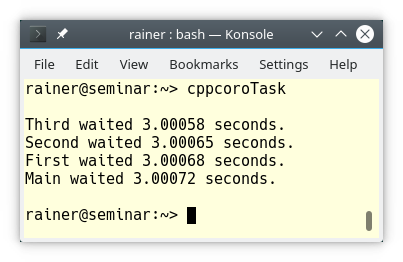
\includegraphics[width=0.8\textwidth]{content/5/chapter8/images/1.png}\\
Coroutines first sleeping
\end{center}

Let’s vary the program a little. What happens if the coroutines sleep after the co\_await call?

\hspace*{\fill} \\ %插入空行
\noindent
Coroutines first waiting
\begin{lstlisting}[style=styleCXX]
// cppcoroTask2.cpp

#include <chrono>
#include <iostream>
#include <string>
#include <thread>

#include <cppcoro/sync_wait.hpp>
#include <cppcoro/task.hpp>

using std::chrono::high_resolution_clock;
using std::chrono::time_point;
using std::chrono::duration;

using namespace std::chrono_literals;

auto getTimeSince(const time_point<::high_resolution_clock>& start) {

	auto end = high_resolution_clock::now();
	duration<double> elapsed = end - start;
	return elapsed.count();

}
cppcoro::task<> third(const time_point<high_resolution_clock>& start) {

	std::cout << "Third waited " << getTimeSince(start) << " seconds." << '\n';
	std::this_thread::sleep_for(1s);
	co_return;

}

cppcoro::task<> second(const time_point<high_resolution_clock>& start) {

	auto thi = third(start);
	co_await thi;
	
	std::cout << "Second waited " << getTimeSince(start) << " seconds." << '\n';
	std::this_thread::sleep_for(1s);

}

cppcoro::task<> first(const time_point<high_resolution_clock>& start) {

	auto sec = second(start);
	co_await sec;
	
	std::cout << "First waited " << getTimeSince(start) << " seconds." << '\n';
	std::this_thread::sleep_for(1s);

}

int main() {

	std::cout << '\n';
	
	auto start = ::high_resolution_clock::now();
	
	cppcoro::sync_wait(first(start));
	
	std::cout << "Main waited " << getTimeSince(start) << " seconds." << '\n';
	
	std::cout << '\n';

}
\end{lstlisting}

You may have guessed it. The main function waits 3 seconds, but each iteratively-invoked coroutine one second less.

The next coroutine that cppcoro provides is a generator<T>.

\hspace*{\fill} \\ %插入空行
\noindent
\textbf{8.1.1.1.2\hspace{0.2cm} generator<T>}

Here is cppcoro’s definition of a generator:

\begin{itemize}
\item 
A generator represents a coroutine type that produces a sequence of values of type T, where values are produced lazily and synchronously.
\end{itemize}

Without further ado, the program cppcoroGenerator.cpp demonstrates two generators in action.

\hspace*{\fill} \\ %插入空行
\noindent
Use of two generators
\begin{lstlisting}[style=styleCXX]
// cppcoroGenerator.cpp

#include <iostream>
#include <cppcoro/generator.hpp>

cppcoro::generator<char> hello() {
	co_yield 'h';
	co_yield 'e';
	co_yield 'l';
	co_yield 'l';
	co_yield 'o';
}

cppcoro::generator<const long long> fibonacci() {
	long long a = 0;
	long long b = 1;
	while (true) {
		co_yield b;
		auto tmp = a;
		a = b;
		b += tmp;
	}
}

int main() {

	std::cout << '\n';
	for (auto c: hello()) std::cout << c;
	
	std::cout << "\n\n";
	
	for (auto i: fibonacci()) {
		if (i > 1'000'000) break;
		std::cout << i << " ";
	}
	
	std::cout << "\n\n";

}
\end{lstlisting}

The first coroutine hello returns on request the next character and the coroutine fibonacci the next fibonacci number. fibonacci creates an infinite data stream. What happens in line 33? The range-based for loop triggers the execution of the coroutine. The first iteration starts the coroutines, returns the value at co\_yield b (line 18), and pauses. Subsequent calls of the range-based for loop resume the coroutine fibonacci and return the next fibonacci number.

\begin{center}
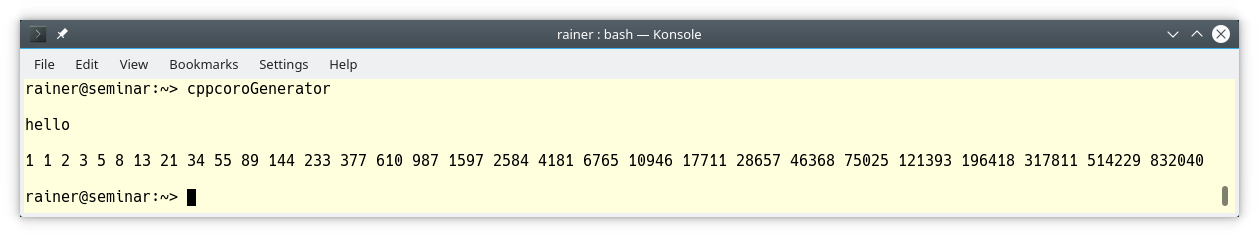
\includegraphics[width=0.8\textwidth]{content/5/chapter8/images/2.png}\\
Executing two generators
\end{center}

cppcoro provides more awaitable types.

\hspace*{\fill} \\ %插入空行
\noindent
\textbf{8.1.1.2\hspace{0.2cm} Awaitable Types}

cppcoro supports various awaitable types:

\begin{itemize}
\item 
single\_consumer\_event

\item 
single\_consumer\_async\_auto\_reset\_event

\item 
async\_mutex

\item 
async\_manual\_reset\_event

\item 
async\_auto\_reset\_event

\item 
async\_latch

\item 
sequence\_barrier

\item 
multi\_producer\_sequencer

\item 
single\_producer\_sequencer
\end{itemize}

I want to have a closer look at the awaitables single\_consumer\_event and async\_mutex.

\hspace*{\fill} \\ %插入空行
\noindent
\textbf{8.1.1.2.1\hspace{0.2cm} single\_consumer\_event}

The single\_consumer\_event is, according to the documentation, a simple manual-reset event type that supports only a single coroutine awaiting it at a time. single\_consumer\_event provides a new way for the one-time synchronization of threads.

\hspace*{\fill} \\ %插入空行
\noindent
One-time thread synchronization with cppcoro
\begin{lstlisting}[style=styleCXX]
// cppcoroProducerConsumer.cpp

#include <cppcoro/single_consumer_event.hpp>
#include <cppcoro/sync_wait.hpp>
#include <cppcoro/task.hpp>

#include <future>
#include <iostream>
#include <string>
#include <thread>
#include <chrono>

cppcoro::single_consumer_event event;

cppcoro::task<> consumer() {

	auto start = std::chrono::high_resolution_clock::now();
	
	co_await event; // suspended until some thread calls event.set()
	
	auto end = std::chrono::high_resolution_clock::now();
	std::chrono::duration<double> elapsed = end - start;
	std::cout << "Consumer waited " << elapsed.count() << " seconds." << '\n';
	
	co_return;
}

void producer() {

	using namespace std::chrono_literals;
	std::this_thread::sleep_for(2s);
	
	event.set(); // resumes the consumer

}

int main() {

	std::cout << '\n';
	
	auto con = std::async([]{ cppcoro::sync_wait(consumer()); });
	auto prod = std::async(producer);
	
	con.get(), prod.get();
	
	std::cout << '\n';

}
\end{lstlisting}

The code should be self-explanatory. The consumer (line 41) and the producer (line 42) run in their thread. The call cppcoro::sync\_wait(consumer()) (line 41) serves as a top-level task because the main function cannot be a coroutine. The call waits until the coroutine consumer is done. The coroutine consumer waits in the call co\_await event (line 19) until someone calls event.set() (line 33). The function producer sends its event after a sleep of two seconds.

\begin{center}
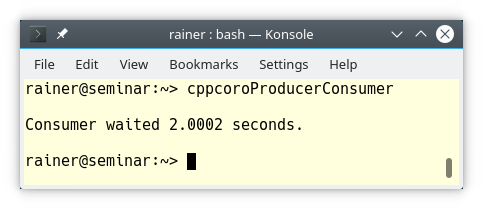
\includegraphics[width=0.8\textwidth]{content/5/chapter8/images/3.png}\\
One-time thread synchronization with cppcoro
\end{center}

cppcoro also supports a \href{https://en.cppreference.com/w/cpp/named_req/Mutex}{mutex}.

\hspace*{\fill} \\ %插入空行
\noindent
\textbf{8.1.1.2.2\hspace{0.2cm} async\_mutex}

A mutex such as cppcoro::async\_mutex is a synchronization mechanism to protect shared data from being accessed by multiple threads simultaneously.

\hspace*{\fill} \\ %插入空行
\noindent
Mutual exclusion with cppcoro
\begin{lstlisting}[style=styleCXX]
// cppcoroMutex.cpp

#include <cppcoro/async_mutex.hpp>
#include <cppcoro/sync_wait.hpp>
#include <cppcoro/task.hpp>

#include <iostream>
#include <thread>
#include <vector>


cppcoro::async_mutex mutex;

int sum{};

cppcoro::task<> addToSum(int num) {
	cppcoro::async_mutex_lock lockSum = co_await mutex.scoped_lock_async();
	sum += num;

}

int main() {

	std::cout << '\n';
	
	std::vector<std::thread> vec(10);
	
	for(auto& thr: vec) {
		thr = std::thread([]{
		for(int n = 0; n < 10; ++n) cppcoro::sync_wait(addToSum(n)); } );
	}
	
	for(auto& thr: vec) thr.join();
	
	std::cout << "sum: " << sum << '\n';
	
	std::cout << '\n';

}
\end{lstlisting}

Line 26 creates ten threads. Each thread adds the numbers 0 to 9 to the shared sum variable (line 14). The function addToSum is the coroutine. The coroutine waits in the expression co\_await mutex.scoped\_lock\_async() (line 17) until the mutex is acquired. The coroutine that waits for the mutex is not blocked but suspended. The previous lock holder resumes the waiting coroutine in its unlock call. As the name suggests, the mutex stays locked until the end of its scope (line 20).

\begin{center}
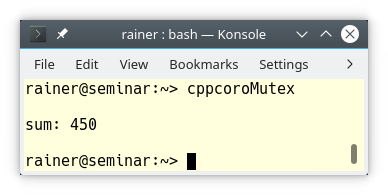
\includegraphics[width=0.8\textwidth]{content/5/chapter8/images/4.png}\\
Mutual exclusion with cppcoro
\end{center}

\hspace*{\fill} \\ %插入空行
\noindent
\textbf{8.1.1.3\hspace{0.2cm} Functions}

There are more interesting functions to handle awaitables.

\begin{itemize}
\item 
sync\_wait()

\item 
when\_all()

\item 
when\_all\_ready()

\item 
fmap()

\item 
schedule\_on()

\item 
resume\_on()
\end{itemize}

The function when\_all creates an awaitable that waits for all its input-awaitables, and returns an aggregate of their individual results.

The following example should give you the first impression:

\hspace*{\fill} \\ %插入空行
\noindent
Waiting for all awaitables with when\_all
\begin{lstlisting}[style=styleCXX]
// cppcoroWhenAll.cpp

#include <chrono>
#include <iostream>
#include <thread>

#include <cppcoro/sync_wait.hpp>
#include <cppcoro/task.hpp>
#include <cppcoro/when_all.hpp>

using namespace std::chrono_literals;

cppcoro::task<std::string> getFirst() {
	std::this_thread::sleep_for(1s);
	co_return "First";
}

cppcoro::task<std::string> getSecond() {
	std::this_thread::sleep_for(1s);
	co_return "Second";
}

cppcoro::task<std::string> getThird() {
	std::this_thread::sleep_for(1s);
	co_return "Third";
}


cppcoro::task<> runAll() {

	auto[fir, sec, thi] = co_await cppcoro::when_all(getFirst(), getSecond(),
	getThird());
	
	std::cout << fir << " " << sec << " " << thi << '\n';

}

int main() {

	std::cout << '\n';
	
	auto start = std::chrono::steady_clock::now();
	
	cppcoro::sync_wait(runAll());
	
	std::cout << '\n';
	
	auto end = std::chrono::high_resolution_clock::now();
	std::chrono::duration<double> elapsed = end - start;
	std::cout << "Execution time " << elapsed.count() << " seconds." << '\n';
	
	std::cout << '\n';

}
\end{lstlisting}

The top-level task cppcoro::sync\_wait(runAll()) (line 44) awaits the awaitable runAll, which awaits the awaitables getFirst, getSecond, and getThird (line 31). The awaitables runAll, getFirst, getSecond, and getThird are coroutines. Each of the get functions sleeps for one second (line 14, 19, and 24 ). Three times one second makes three seconds. This is the time the call cppcoro::sync\_wait(runAll()) waits for the coroutines. Line 49 displays the time duration.

\begin{center}
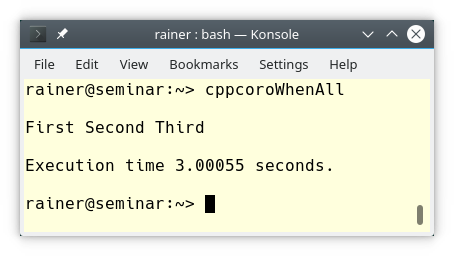
\includegraphics[width=0.8\textwidth]{content/5/chapter8/images/5.png}\\
Waiting for all awaitables with when\_all
\end{center}

You can combine when\_all with thread pools in cpp

\hspace*{\fill} \\ %插入空行
\noindent
\textbf{8.1.1.4\hspace{0.2cm} static\_thread\_pool}

static\_thead\_pool schedules work on a fixed-size pool of threads.

cppcoro::static\_thread\_pool can be invoked with and without a number. The number stands for the number of threads that are created. If you don’t specify a number, the C++11 function std::thread::hardware\_concurrency() is used. \href{https://en.cppreference.com/w/cpp/thread/thread/hardware_concurrency}{std::thread::hardware\_concurrency} gives you a hint for the number of hardware threads supported by your system. This may be the number of processors or cores you have.

Let me try it out. The following example is based on the previous one cppcoroWhenAll.cpp using the awaitable when\_any. This time, the coroutines are executed concurrently.

\hspace*{\fill} \\ %插入空行
\noindent
Waiting for concurrently running awaitables with when\_all
\begin{lstlisting}[style=styleCXX]
// cppcoroWhenAllOnThreadPool.cpp

#include <chrono>
#include <iostream>
#include <thread>

#include <cppcoro/sync_wait.hpp>
#include <cppcoro/task.hpp>
#include <cppcoro/static_thread_pool.hpp>
#include <cppcoro/when_all.hpp>


using namespace std::chrono_literals;

cppcoro::task<std::string> getFirst() {
	std::this_thread::sleep_for(1s);
	co_return "First";
}

cppcoro::task<std::string> getSecond() {
	std::this_thread::sleep_for(1s);
	co_return "Second";
}

cppcoro::task<std::string> getThird() {
	std::this_thread::sleep_for(1s);
	co_return "Third";
}

template <typename Func>
cppcoro::task<std::string> runOnThreadPool(cppcoro::static_thread_pool& tp,
                                           Func func) {
	co_await tp.schedule();
	auto res = co_await func();
	co_return res;
}

cppcoro::task<> runAll(cppcoro::static_thread_pool& tp) {

	auto[fir, sec, thi] = co_await cppcoro::when_all(
		runOnThreadPool(tp, getFirst),
		runOnThreadPool(tp, getSecond),
		runOnThreadPool(tp, getThird));
	
	std::cout << fir << " " << sec << " " << thi << '\n';

}

int main() {

	std::cout << '\n';
	
	auto start = std::chrono::steady_clock::now();
	
	cppcoro::static_thread_pool tp;
	cppcoro::sync_wait(runAll(tp));
	
	std::cout << '\n';
	
	auto end = std::chrono::high_resolution_clock::now();
	std::chrono::duration<double> elapsed = end - start;
	std::cout << "Execution time " << elapsed.count() << " seconds." << '\n';
	
	std::cout << '\n';

}
\end{lstlisting}

This is the crucial difference with the previous program cppcoroWhenAll.cpp. At line 55, I create a thread pool tp and use it as an argument for the function runAll(tp) (line 56). The function runAll uses the thread pool to start the coroutines concurrently. Thanks to structured binding (line 40), the values of each coroutine can be easily aggregated and assigned to a variable. In the end, the main function takes one instead of three seconds.

\begin{center}
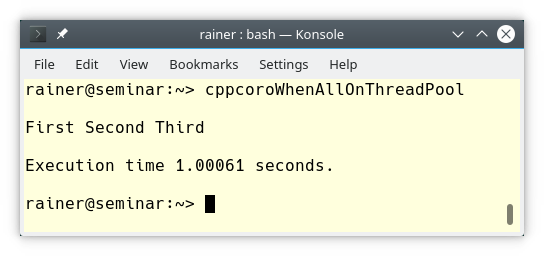
\includegraphics[width=0.8\textwidth]{content/5/chapter8/images/6.png}\\
Waiting for all awaitables with when\_all
\end{center}

\subsubsubsection{8.1.2\hspace{0.2cm} Modularized Standard Library for Modules}

Maybe you’d like to stop using Standard Library headers? Microsoft supports modules for all STL headers according to the C++ proposal \href{http://www.open-std.org/JTC1/SC22/WG21/docs/papers/2017/p0581r0.pdf}{P0541}. Microsoft’s implementation gives you the first idea of how a modularized standard library for modules could look like. Here is what I have found in the post \href{https://devblogs.microsoft.com/cppblog/cpp-modules-in-visual-studio-2017/}{Using C++ Modules in Visual Studio 2017} from the Microsoft C++ team blog.

\hspace*{\fill} \\ %插入空行
\noindent
\textbf{8.1.2.1\hspace{0.2cm} C++ modules in Visual Studio 2017}

\begin{itemize}
\item 
std.regex provides the content of the header <regex>

\item 
std.filesystem provides the content of the header <experimental/filesystem>

\item 
std.memory provides the content of the header <memory>

\item 
std.threading provides the contents of headers <atomic>, <condition\_variable>, <future>, <mutex>, <shared\_mutex>, and <thread>

\item 
std.core provides everything else in the C++ Standard Library
\end{itemize}

To use the Microsoft Standard Library modules, you have to specify the exception handling model (/EHsc) and the multithreading library (/MD). Additionally, you have to use the flags /std:c++latest and /experimental:module.

In the section on modules, I used the following module definition.

\hspace*{\fill} \\ %插入空行
\noindent
A module definition with a global module fragment
\begin{lstlisting}[style=styleCXX]
// math1.ixx

module;

#include <numeric>
#include <vector>

export module math;

export int add(int fir, int sec){
	return fir + sec;
}

export int getProduct(const std::vector<int>& vec) {
	return std::accumulate(vec.begin(), vec.end(), 1, std::multiplies<int>());
}
\end{lstlisting}

This module definition can directly be refactored using the modularized standard library. You have to replace the headers <numeric> and <vector> with the module std.core.

\hspace*{\fill} \\ %插入空行
\noindent
Importing the module std.core into the interface file
\begin{lstlisting}[style=styleCXX]
// math2.ixx
module;

export module math;

import std.core;

export int add(int fir, int sec){
	return fir + sec;
}

export int getProduct(const std::vector<int>& vec) {
	return std::accumulate(vec.begin(), vec.end(), 1, std::multiplies<int>());
}
\end{lstlisting}

Furthermore, you must use the module std.core instead of the standard header files:

\hspace*{\fill} \\ %插入空行
\noindent
Importing the module std.core into the client program
\begin{lstlisting}[style=styleCXX]
// client2.cpp

import math;
import std.core;

int main() {
	
	std::cout << '\n';
	
	std::cout << "add(2000, 20): " << add(2000, 20) << '\n';
	
	std::vector<int> myVec{1, 2, 3, 4, 5, 6, 7, 8, 9, 10};
	
	std::cout << "getProduct(myVec): " << getProduct(myVec) << '\n';
	
	std::cout << '\n';
}
\end{lstlisting}

The program produces the expected output:

\begin{center}
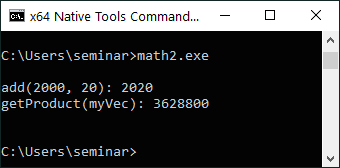
\includegraphics[width=0.8\textwidth]{content/5/chapter8/images/7.png}\\
Using the module std.core on Windows
\end{center}

\subsubsubsection{8.1.3\hspace{0.2cm} Executors}

Executors have quite a history in C++. The discussion began at early as 2010. For the details, Detlef Vollmann gives in his presentation \href{http://www.vollmann.ch/en/presentations/executors2018.pdf}{Finally Executors for C++} an excellent overview.

My introduction to executors is mainly based on the proposals for the design of executors \href{http://www.open-std.org/jtc1/sc22/wg21/docs/papers/2018/p0761r2.pdf}{P0761}, and their formal description \href{http://open-std.org/JTC1/SC22/WG21/docs/papers/2018/p0443r7.html}{P0443}. I also refer to the relatively new \href{http://open-std.org/JTC1/SC22/WG21/docs/papers/2018/p1055r0.pdf}{Modest Executor Proposal P1055}.

First of all. What are Executors?

Executors are the basic building blocks for execution in C++ and fulfill a similar role for execution, such as allocators for the containers in C++. Many proposals for executors are published, and many design decisions are still open. They should be part of C++23, but can probably be used much earlier to extend the C++ standard.

An executor consists of rules about where, when, and how to run a callable.

\begin{itemize}
\item 
Where: The callable may run on an internal or external processor, and that the result is read back from the internal or external processor.

\item 
When: The callable may run immediately or just be scheduled.

\item 
How: The callable may run on a CPU or GPU or even be executed in a vectorized way
\end{itemize}

The concurrency and parallelism features of C++ heavily depend on executors as building blocks for execution. This dependency holds for existing concurrency features, such as the \href{https://www.modernescpp.com/index.php/parallel-algorithm-of-the-standard-template-library}{parallel algorithms of the Standard Template Library}, but also for new concurrency features, such as \href{https://www.modernescpp.com/index.php/std-future-extensions}{latches and barriers, coroutines, the network library, extended futures}, \href{https://www.modernescpp.com/index.php/transactional-memory}{transactional memory}, or \href{https://www.modernescpp.com/index.php/task-blocks}{task blocks}.

\hspace*{\fill} \\ %插入空行
\noindent
\textbf{8.1.3.1\hspace{0.2cm} First Examples}

The following code snippets should give you a first impression of executors.

\hspace*{\fill} \\ %插入空行
\noindent
\textbf{8.1.3.1.1\hspace{0.2cm} Using an Executor}

\begin{itemize}
\item 
The promise std::async

\hspace*{\fill} \\ %插入空行
\noindent
std::async uses an executor
\begin{lstlisting}[style=styleCXX]
// get an executor through some means
my_executor_type my_executor = ...

// launch an async using my executor
auto future = std::async(my_executor, [] {
	std::cout << "Hello world, from a new execution agent!" < '\n';
});
\end{lstlisting}

\item 
The STL algorithm std::for\_each

\hspace*{\fill} \\ %插入空行
\noindent
std::for\_each uses an executor
\begin{lstlisting}[style=styleCXX]
// get an executor through some means
my_executor_type my_executor = ...

// execute a parallel for_each "on" my executor
std::for_each(std::execution::par.on(my_executor),
			  data.begin(), data.end(), func);
\end{lstlisting}
\end{itemize}

\hspace*{\fill} \\ %插入空行
\noindent
\textbf{8.1.3.1.2\hspace{0.2cm} Obtaining an Executor}

There are various ways to obtain an executor.

\begin{itemize}
\item 
From the execution context static\_thread\_pool

\hspace*{\fill} \\ %插入空行
\noindent
An exector from the static\_thread\_pool
\begin{lstlisting}[style=styleCXX]
// create a thread pool with 4 threads
static_thread_pool pool(4);

// get an executor from the thread pool
auto exec = pool.executor();

// use the executor on some long-running task
auto task1 = long_running_task(exec);
\end{lstlisting}

\item 
From the system executor
\end{itemize}

The system executor is the default executor used if not specified otherwise.

\begin{itemize}
\item 
From an executor adapter

\hspace*{\fill} \\ %插入空行
\noindent
Adapting an executor
\begin{lstlisting}[style=styleCXX]
// get an executor from a thread pool
auto exec = pool.executor();

// wrap the thread pool's executor in a logging_executor
logging_executor<decltype(exec)> logging_exec(exec);

// use the logging executor in a parallel sort
std::sort(std::execution::par.on(logging_exec), my_data.begin(), my_data.end());
\end{lstlisting}

logging\_executor is a wrapper for the pool executor.
\end{itemize}

\hspace*{\fill} \\ %插入空行
\noindent
\textbf{8.1.3.2\hspace{0.2cm} Goals of an Executor Concept}

What are the goals of an executor concept according to proposal \href{http://open-std.org/JTC1/SC22/WG21/docs/papers/2018/p1055r0.pdf}{P1055}?

\begin{itemize}
\item 
Batchable: control the trade-off between the cost of the transition of the callable and its size.

\item 
Heterogenous: allow the callable to run on heterogeneous contexts and get the result back.

\item 
Orderable: specify the order in which the callables are invoked. The goal includes ordering guarantees such as LIFO (Last In, First Out), FIFO (First In, First Out) execution, priority or time constraints, or even sequential execution.

\item 
Controllable: the callable has to be targetable to a specific compute resource, deferred, or even canceled.

\item 
Continuable: for non-blocking submission of work units, signals from the work units are needed. These signals have to indicate, whether the result is available, whether an error occurred, when the callable is done or if the callee wants to cancel the callable. The explicit starting of the callable or the stopping of the staring should also be possible.

\item 
Layerable: hierarchies allow new capabilities to be added without increasing the complexity of the simpler use-cases.

\item 
Usable: ease of use for the implementer and the user should be the main goal.
 
\item 
Composable: allows a user to extend the executors for features that are not part of the standard.

\item 
Minimal: nothing should exist on the executor concepts that could be added externally in a library on top of the concept.
\end{itemize}

\hspace*{\fill} \\ %插入空行
\noindent
\textbf{8.1.3.3\hspace{0.2cm} Execution Function}

An executor provides one or more execution functions for creating execution agents from a callable. An executor has to support at least one of the six following functions.

\begin{center}
Exuction functions of a executor
\end{center}

\begin{table}[H]
\centering
\begin{tabular}{lll}
\textbf{Member function} & \textbf{Cardinality} & \textbf{Direction} \\ \hline
execute                  & single               & oneway             \\
twoway\_execute          & single               & twoway             \\
then\_execute            & single               & then               \\
bulk\_execute            & bulk                 & oneway             \\
bulk\_twoway\_execute    & bulk                 & twoway             \\
bulk\_then\_execute      & bulk                 & then              
\end{tabular}
\end{table}

Each execution function has two properties: cardinality and direction.

\begin{itemize}
\item 
Cardinality:
\begin{itemize}
\item 
single: creates one execution agent

\item 
bulk: creates a group of execution agents
\end{itemize}

\item 
Direction:
\begin{itemize}
\item 
oneway: creates an execution agent and does not return a result

\item
twoway: creates an execution agent and returns a future that can be used to wait for execution to complete

\item
then: creates an execution agent and returns a future that can be used to wait for execution to complete. The execution agent begins execution after a given future becomes ready.
\end{itemize}
\end{itemize}

The next lines give a more formal explanation of the execution functions.

First, I refer to the single cardinality case:

\begin{itemize}
\item 
A oneway execution function is a fire-and-forget job. It’s quite similar to a fire-and-forget future, but it does not automatically block in the destructor of the \href{https://www.modernescpp.com/index.php/the-special-futures}{future}.

\item
A twoway execution function returns you a future which you can use to pick up the result. This behaves similarly to a \href{https://www.modernescpp.com/index.php/promise-and-future}{std::promise} that gives you back the handle to the associated std::future.

\item
A then execution function is a continuation. It gives you back a future, but the execution agent runs only if the provided future is ready.
\end{itemize}

Second, the bulk cardinality case is more complicated. These functions create a group of execution agents, and each of these execution agents calls the given callable. They return the result of a factory and not the result of a single callable f invoked by the execution agents. The user is responsible for disambiguating the right result via this factory.

\hspace*{\fill} \\ %插入空行
\noindent
\textbf{8.1.3.3.1\hspace{0.2cm} execution::require}

How can you be sure that your executor supports the specific execution function?

In the special case, you know it:

\hspace*{\fill} \\ %插入空行
\noindent
An executor using the execution function execute
\begin{lstlisting}[style=styleCXX]
void concrete_context(const my_oneway_single_executor& ex)
{
	auto task = ...;
	ex.execute(task);
}
\end{lstlisting}

In the general case, you can use the function execution::require to ask for it.

\hspace*{\fill} \\ %插入空行
\noindent
An executor requiring a single and twoway execution function
\begin{lstlisting}[style=styleCXX]
template <typename Executor>
void generic_context(const Executor& ex)
{
	auto task = ...;
	
	// ensure .twoway_execute() is available with execution::require()
	execution::require(ex, execution::single, execution::twoway).twoway_execute(task\
	);
}
\end{lstlisting}

In this case, the executor ex has to support single cardinality and twoway direction execution.

\subsubsubsection{8.1.4\hspace{0.2cm} The Network Library}

The network library in C++23 is based on the \href{https://www.boost.org/doc/libs/1_75_0/doc/html/boost_asio.html}{boost::asio} library from Christopher M. Kohlhoff. The library targets the network and low-level I/O programming.

The following components are part of the network library

\begin{itemize}
\item 
TCP, UDP, and multicast

\item 
Client/Server applications

\item 
Scalability for more concurrent connections

\item 
IPv4 and IPv6

\item 
Name resolution (DNS)

\item 
Clocks
\end{itemize}

However, the following components are not part of the network library:

\begin{itemize}
\item 
Implementation of network protocols such as HTTP, SMTP, or FTP

\item 
Encryption (SSL or TLS)

\item 
Operating specific multiplexing interfaces, such as select or poll

\item 
Support for realtime

\item 
TCP/IP protocols like ICMP
\end{itemize}

Thanks to the network library, you can directly implement an echo server.

\hspace*{\fill} \\ %插入空行
\noindent
A simple echo server
\begin{lstlisting}[style=styleCXX]
template <typename Iterator>
void uppercase(Iterator begin, Iterator end) {
	std::locale loc("");
	for (Iterator iter = begin; iter != end; ++iter)
	*iter = std::toupper(*iter, loc);
}

void sync_connection(tcp::socket& socket) {
	try {
		std::vector<char> buffer_space(1024);
		while (true) {
			std::size_t length = socket.read_some(buffer(buffer_space));
			uppercase(buffer_space.begin(), buffer_space.begin() + length);
			write(socket, buffer(buffer_space, length));
		}
	}
	catch (std::system_error& e) {
		// ...
	}
}
\end{lstlisting}

The server gets the client socket socket socket (line 8), reads the text (line 12), transforms the text into capital letters (line 13), and sends the text back to the client (line 14).

The boost library has more examples of chat or HTTP servers. Additionally, the server can run synchronously - such as presented in the program - or asynchronously.






















